\projectstart{p3}{P3}{Acceleròmetre 3D}

\section{Objectius}

En aquesta pràctica es programarà el mòdul de codi que farà la comunicació
amb l'acceleròmetre 3D SPI que porta integrada la placa.

Es començarà explicant com l'acceleròmetre està connectat al microcontrolador,
el funcionament del bus que utilitza (SPI) i l'us des del codi, i després
la lectura i escriptura dels registres de l'acceleròmetre i per a què serveix
cadascun.

\section{Desenvolupament}


\subsection{Funcionament de l’acceleròmetre i connexió amb el microcontrolador}

S'explica el funcionament general de l'acceleròmetre, la posició dels eixos de mesura
i les diferències entre les places noves i les velles, les connexions amb el
microcontrolador i la funció de cadascun dels senyals.

A continuació s'explica com els pins GPIO es poden reconfigurar en una de fins a setze
\emph{funcions alternatives} (AFs); en el nostre cas la funció AF5 permet tenir accés a
\textsf{SPI1\_SCL}, \textsf{SPI1\_MISO} i \textsf{SPI1\_MOSI} des de \textsf{PA5}, \textsf{PA6}
i \textsf{PA7} respectivament. Els pins \textsf{INT1} i \textsf{INT2} no es faran servir
en aquesta pràctica, i el pin de \emph{chip select} s'ha de configurar com a sortida \emph{push-pull}
ja que el controlarem manualment. Tot això ja es fa des de \fname{baseInit}.

Es detallen els registres de l'acceleròmetre i s'explica el funcionament de \textsf{Who\_Am\_I}
(\mintinline{c}|0x0F|) i \textsf{Ctrl\_Reg1} (\mintinline{c}|0x20|).

\subsection{Descripció del bus SPI}

% FIXME: posar algun cronograma o algo :)

S'explica l'estructura de busos i rellotges del microcontrolador i la necessitat d'encendre el
perifèric SPI1 mitjançant el RCC, ja que per defecte està apagat per reduir el consum.

Llavors s'explica el funcionament del protocol SPI, i l'us del perifèric SPI. S'explica com
s'ha de configurar i com es fan les transferències de 8~bits.

Per començar es demana com a estudi previ, determinar el valor que hem de programar al divisor de
rellotge (del que s'obté \textsf{SCL}) per obtenir la freqüència adequada (segons les especificacions
de l'acceleròmetre):

%previ
Segons el datasheet de l'acceleròmetre (secció~23.1, pàg.~12), la freqüència de rellotge
de l'SPI no ha de superar \(f_c(SPC) = \SI{10}{\mega\hertz}\).

Partint del rellotge base \(f_{clk} = \SI{84}{\mega\hertz}\), el valor més alt que podem posar al
divisor és \(f_{clk} / 16\), el que ens dona una freqüència d'SPI de \SI{5.25}{\mega\hertz}.
Per tant, BR[2:0] s'ha d'establir a \mintinline{c}|0b011|~(3).
%/previ


\subsection{Configuració del bus SPI}

S'expliquen amb més detall els registres pertinents a la configuració i les transferències,
i llavors es demana com a segon estudi previ, implementar una funció \fname{initAccel} que
realitzi tota la la inicialització requerida per a l'accés a l'acceleròmetre
(encendre SPI1, configurar-lo, etc.):

%previ
\begin{minted}[mathescape]{c}
void initAccel(void) {
    // Power on SPI peripheral
    RCC->APB2ENR |= RCC_APB2ENR_SPI1EN;

    // Configure CS pin as push-pull output with '1'
    GPIO_ModePushPull(LIS_CS_PORT, LIS_CS_PAD);
    LIS_CS_PORT->BSRR.H.set = LIS_CS_BIT;

    // Configure CR1
    uint16_t cr1 = SPI1->CR1;
    // Set CPOL = CPHA = 1
    cr1 |= SPI_CR1_CPOL | SPI_CR1_CPHA;
    // Set BR[2:0] to 011 $f_{clk}/16$, which sets a baudrate of $\SI{5.25}{\mega\hertz}$
    cr1 = (cr1 & (~SPI_CR1_BR)) | (0b011 * SPI_CR1_BR_0);
    // Set DFF = 0 (8-bit data)
    cr1 &= ~SPI_CR1_DFF;
    // Set SSM = SSI = 1 (manage CS in software)
    cr1 |= SPI_CR1_SSM | SPI_CR1_SSI;
    // Set MSTR = 1 (act as a master)
    cr1 |= SPI_CR1_MSTR;
    // Set SPE = 1 (enable peripheral)
    cr1 |= SPI_CR1_SPE;
    // Write register
    SPI1->CR1 = cr1;
}
\end{minted}
\vskip -1em
%/previ

% FIXME: voluntari, s'escriu el registre un unic cop!

Es demana que s'importin els fitxers \filename{accel.c} i \filename{accel.h} al projecte
i que s'afegeixi el primer al \filename{Makefile} (\commit{4181e747ed29d63977c9d38a8dc95eed7c0d47e8}).


\subsection{\label{sub:p3-whoami} Lectura de dades de l’acceleròmetre}

S'explica a més alt nivell (específic de l'acceleròmetre) com fer una transferència
de lectura d'un dels seus registres. Es composa d'una primera transmissió SPI on
l'acceleròmetre no entrega res, només llegeix la comanda, i una segona on descarta
l'entrada i ens retorna el valor del registre. Tot això ja està implementat, en la
funció \fname{readAccel}.

\voluntari
Per fer més senzill l'us del mòdul, s'ha editat \filename{accel.h} per afegir constants
per a cada registre de l'acceleròmetre, amb la seva direcció:

\begin{minted}{c}
/************ Public constants **************/

// Register constants

#define LIS_R_WHO_AM_I          0x0F
#define LIS_R_CTRL_REG1         0x20
#define LIS_R_CTRL_REG2         0x21
#define LIS_R_CTRL_REG3         0x22
#define LIS_R_HP_FILTER_RESET   0x23
#define LIS_R_STATUS_REG        0x27
#define LIS_R_OUT_X             0x29
#define LIS_R_OUT_Y             0x2B
#define LIS_R_OUT_Z             0x2D
#define LIS_R_FF_WU_CFG_1       0x30
#define LIS_R_FF_WU_SRC_1       0x31
#define LIS_R_FF_WU_THS_1       0x32
#define LIS_R_FF_WU_DURATION_1  0x33
#define LIS_R_FF_WU_CFG_2       0x34
#define LIS_R_FF_WU_SRC_2       0x35
#define LIS_R_FF_WU_THS_2       0x36
#define LIS_R_FF_WU_DURATION_2  0x37
#define LIS_R_CLICK_CFG         0x38
#define LIS_R_CLICK_SRC         0x39
#define LIS_R_CLICK_THSY_X      0x3B
#define LIS_R_CLICK_THSZ        0x3C
#define LIS_R_CLICK_TIMELIMIT   0x3D
#define LIS_R_CLICK_LATENCY     0x3E
#define LIS_R_CLICK_WINDOW      0x3F
\end{minted}
\vskip -1em

Es demana ara que s'emplenin els continguts de \fname{initAccel} feta anteriorment,
i que es modifiqui \fname{main} perquè cridi a \fname{initAccel} i després faci
servir \fname{readAccel} per llegir el valor del registre \textsf{Who\_Am\_I}
(\mintinline{c}|0x0F|) i mostri el resultat a l'LCD:

\begin{minted}{c}
void accelWhoAmI(void) {
    LCD_ClearDisplay();

    // Read register, convert to string
    int32_t value = readAccel(LIS_R_WHO_AM_I, 0);
    char valueStr [4];
    itoa(value, valueStr, 16);

    // Show in display
    LCD_SendString("Who_Am_I:");
    LCD_GotoXY(0, 1);
    LCD_SendString("0x");
    LCD_SendString(valueStr);
}
\end{minted}
\vskip -1em

\voluntari Més endavant, s'implementa codi per mostrar també el model d'acceleròmetre del
que es disposa, mirant el valor del registre anterior (veure \emph{Ajustaments posteriors}).

El programa es puja a la placa i es comprova que el programa té el comportament esperat,
tant en una placa nova com en una vella. En la figura~\ref{fig:p3-board-whoami} es
pot veure el resultat en una placa vella.

\begin{figure}
  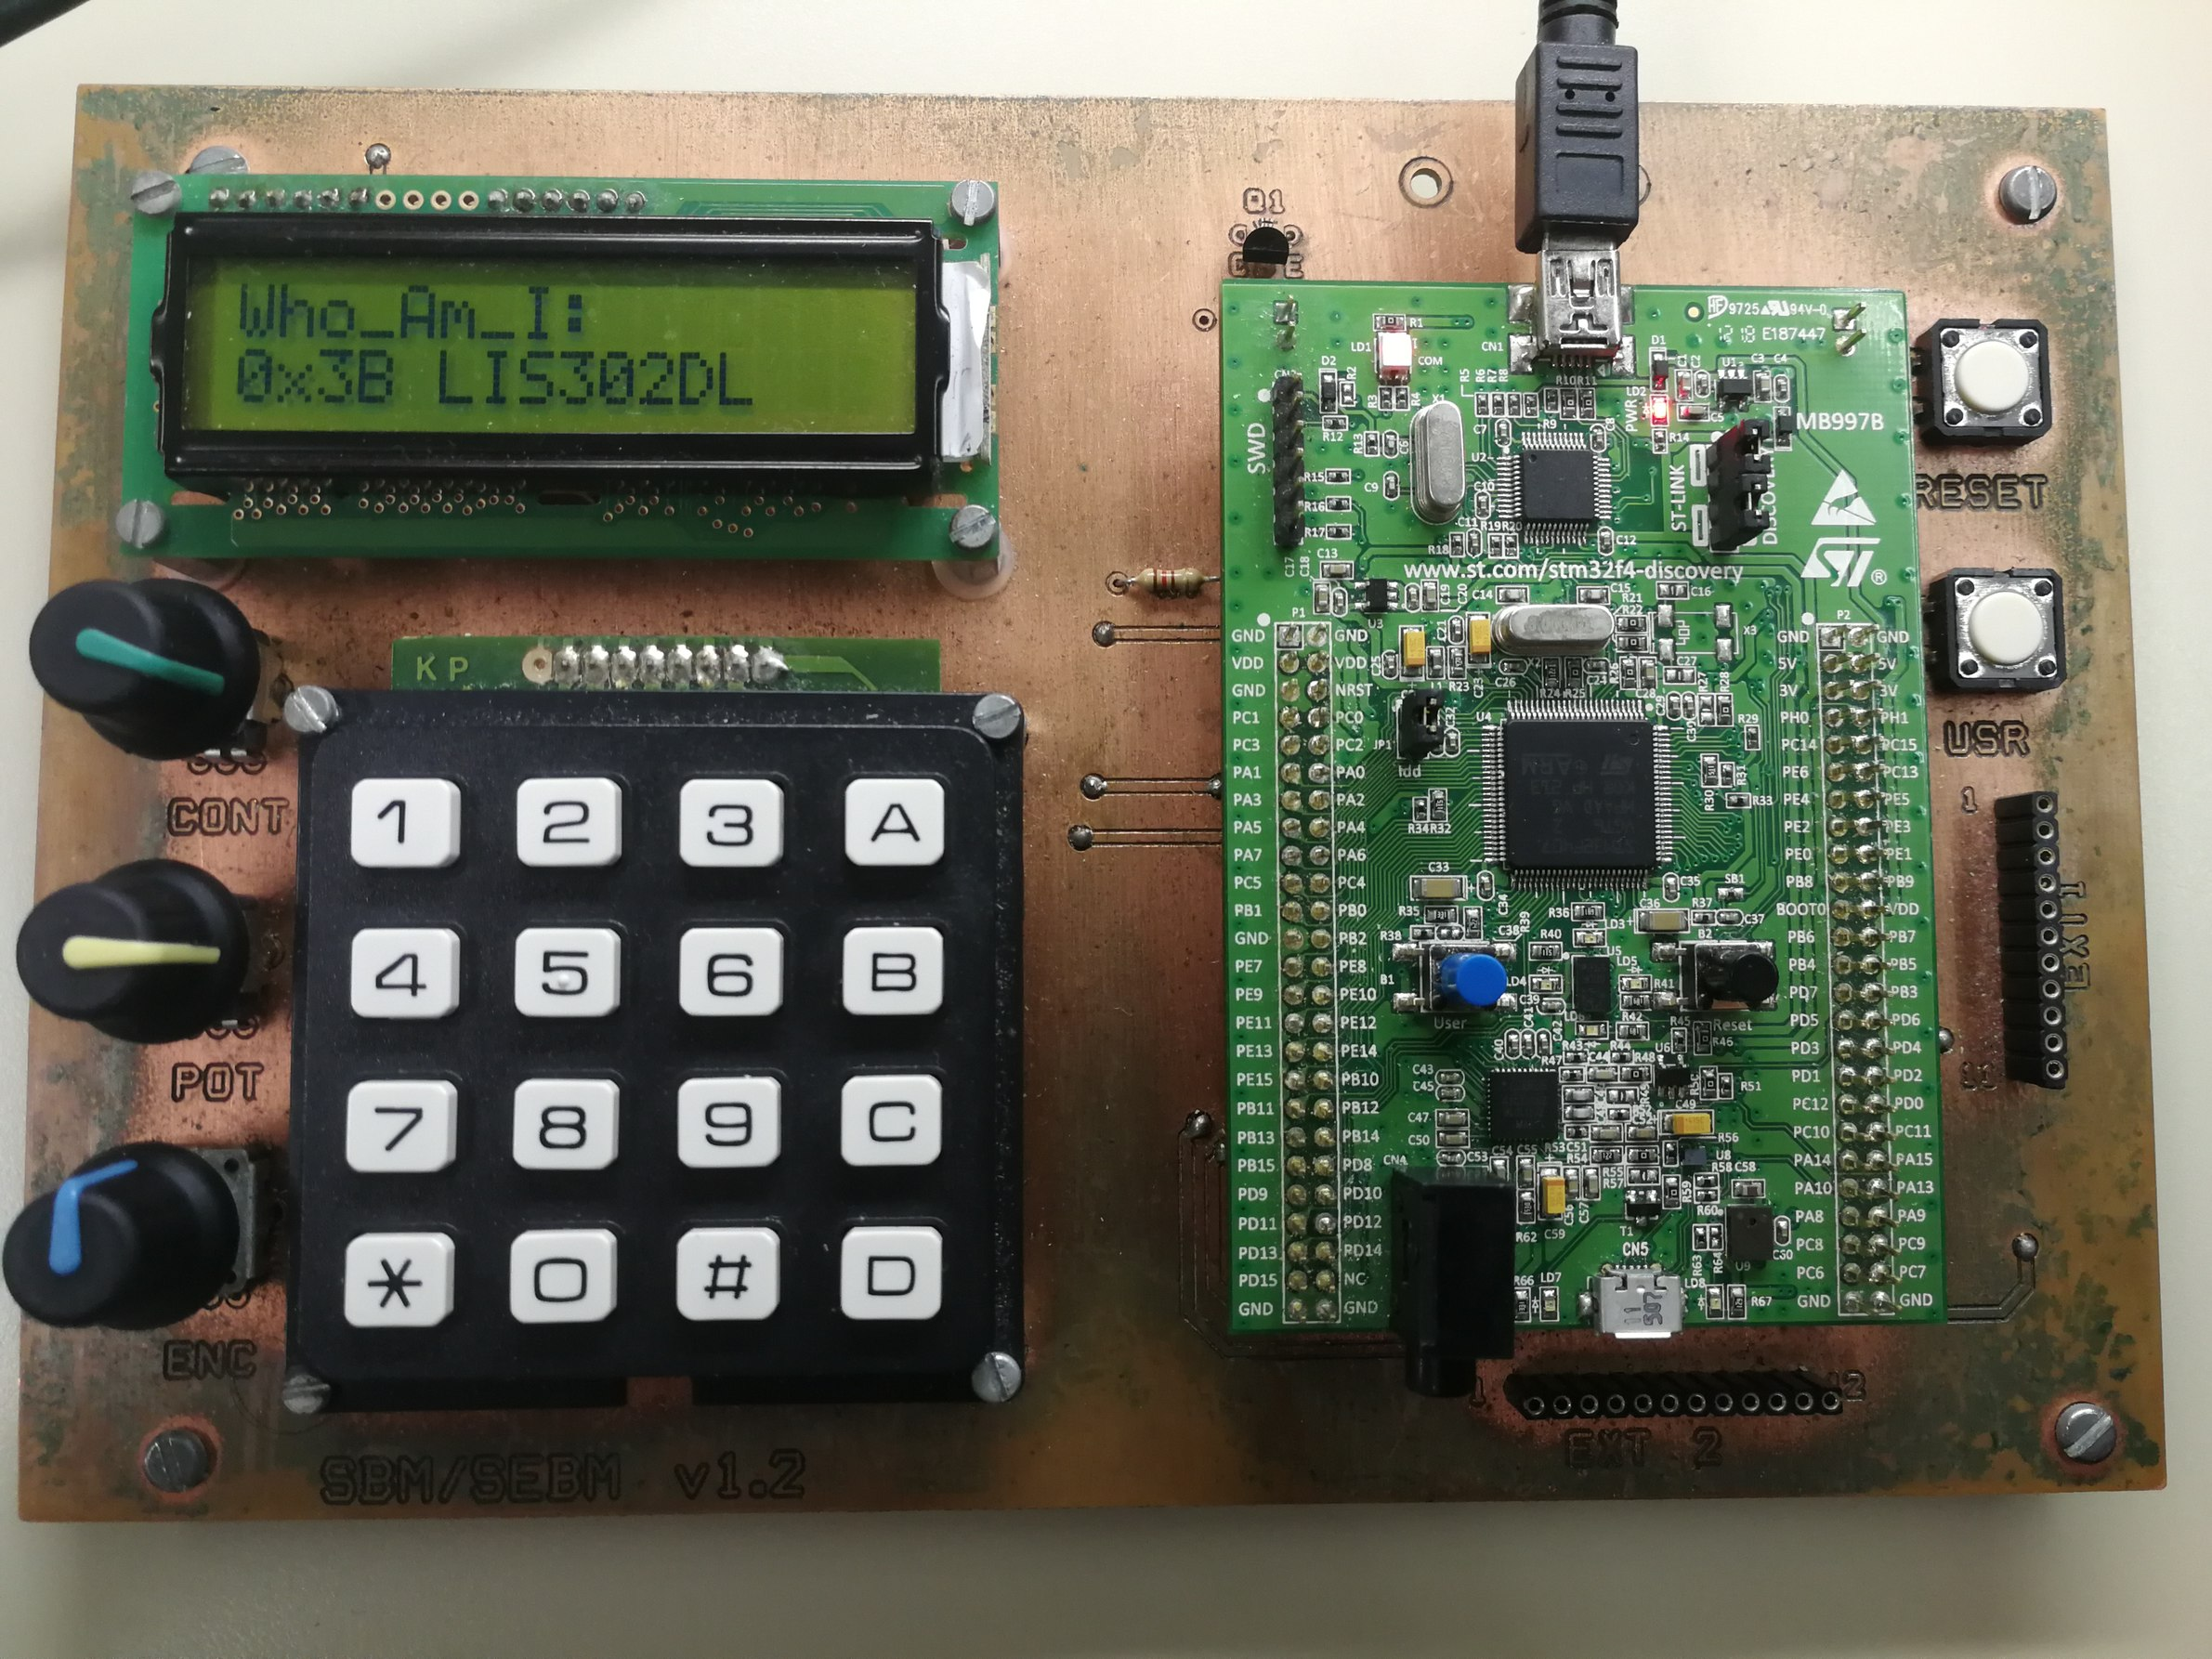
\includegraphics[width=.99\columnwidth]{../photos/board/p3-whoami}
  \caption{ \label{fig:p3-board-whoami} La placa mostrant el valor \textsf{Who\_Am\_I} de l'acceleròmetre i el model. }
\end{figure}

Aquests canvis conformen el \commit{edc28c419c06eecb09acdc6ad45f11e3211a7ac1}.


\subsection{Escriptura de dades a l'acceleròmetre}

A continuació s'explica en primer lloc, la necessitat de treure l'acceleròmetre del
mode \emph{power down} per poder llegir els valors d'acceleració. Per fer-ho, s'ha
de llegir i escriure el registre \textsf{Ctrl\_Reg1} (\mintinline{c}|0x20|) per
posar el bit \textsf{PD} a 1.

\voluntari
Per millorar la qualitat de codi i simplificar-lo, les validacions de la direcció de
registre s'han extret a les funcions \fname{registerIsReserved} i \fname{registerIsReadOnly},
per no repetir el codi dues vegades a \fname{readAccel} i \fname{writeAccel}:

\begin{minted}{c}
static inline int32_t registerIsReserved(int32_t reg) {
    return (reg < 0x0F) ||
           ((reg < 0x20)&&(reg > 0x0F)) ||
           ((reg < 0x27)&&(reg > 0x23)) ||
           ((reg < 0x30)&&(reg > 0x2D));
}

static inline int32_t registerIsReadOnly(int32_t reg) {
    return (reg == LIS_R_WHO_AM_I) || (reg >= 0x23 && reg <= 0x2D) ||
           (reg == LIS_R_CLICK_SRC) || (reg == LIS_R_FF_WU_SRC_2) ||
           (reg == LIS_R_FF_WU_SRC_1);
}
\end{minted}
\vskip -1em

Es demana com a estudi previ, una versió inicial del codi que fa aquesta tasca.

\opcional
Seguint l'apartat opcional, es defineix una funció genèrica per escriure el valor
d'un registre arbitrari. Ja que no tots els registres tenen permesa l'escriptura,
i fer una escriptura quan és el cas pot danyar permanentment l'acceleròmetre,
es demana que la funció comprovi si es tracta d'un registre no legal o només
lectura, i en aquest cas retorni l'error apropiat. La funció s'ha implementat així:

\begin{minted}{c}
// Write an accelerometer register
//      reg   : Number of the register to write
//      val   : Value to write, only 8 lower bits will be used
//
// In case of error returns numbers greater than 1000, otherwise 0
//             1001 : Try to access a reserved register
//             1002 : Try to access a read-only register

int32_t writeAccel(int32_t reg, int32_t val) {
    // Limit the register number to 6 bits 0..63
    // Bit 6 = 0 -> autoincrement disabled
    // Bit 7 = 0 -> write mode
    reg &= 0x3F;

    // Verify it is not a reserved register
    if (registerIsReserved(reg)) return 1001;
    if (registerIsReadOnly(reg)) return 1002;

    // Activates Chip Select
    LIS_CS_PORT->BSRR.H.clear = LIS_CS_BIT;

    // Send command
    SPI1->DR = reg;

    // Small delay before reading the buffer
    DELAY_US(2);

    // Wait to the receiver buffer to fill, and discard value
    while (!((SPI1->SR) & SPI_SR_RXNE));
    SPI1->DR;

    // Send the value
    SPI1->DR = val;

    // Small delay before reading the buffer
    DELAY_US(2);

    // Wait to the receiver buffer to fill, and discard value
    while (!((SPI1->SR) & BIT0));
    SPI1->DR;

    // Deactivates Chip Select
    LIS_CS_PORT->BSRR.H.set = LIS_CS_BIT;

    return 0;
}
\end{minted}
\vskip -1em

El codi demanat en l'estudi previ esdevé llavors:

%previ
\begin{minted}{c}
    // Set PD bit at CTRL_REG1 to 1 Powered
    int32_t ctrl_reg1 = readAccel(LIS_R_CTRL_REG1, 0);
    ctrl_reg1 |= BIT6;
    writeAccel(LIS_R_CTRL_REG1, ctrl_reg1);
\end{minted}
\vskip -1em
%/previ

Es modifica el programa de \fname{main} perquè després d'inicialitzar la placa, LCD
i acceleròmetre, es llegeixi periòdicament el registre d'acceleració Y i es mostri
el valor a la pantalla. En les figures \ref{fig:p3-board-reading-initial} i
\ref{fig:p3-board-reading-tilt} es pot veure el programa funcionant.

\begin{figure}[p] %FIXME: subfigures?
  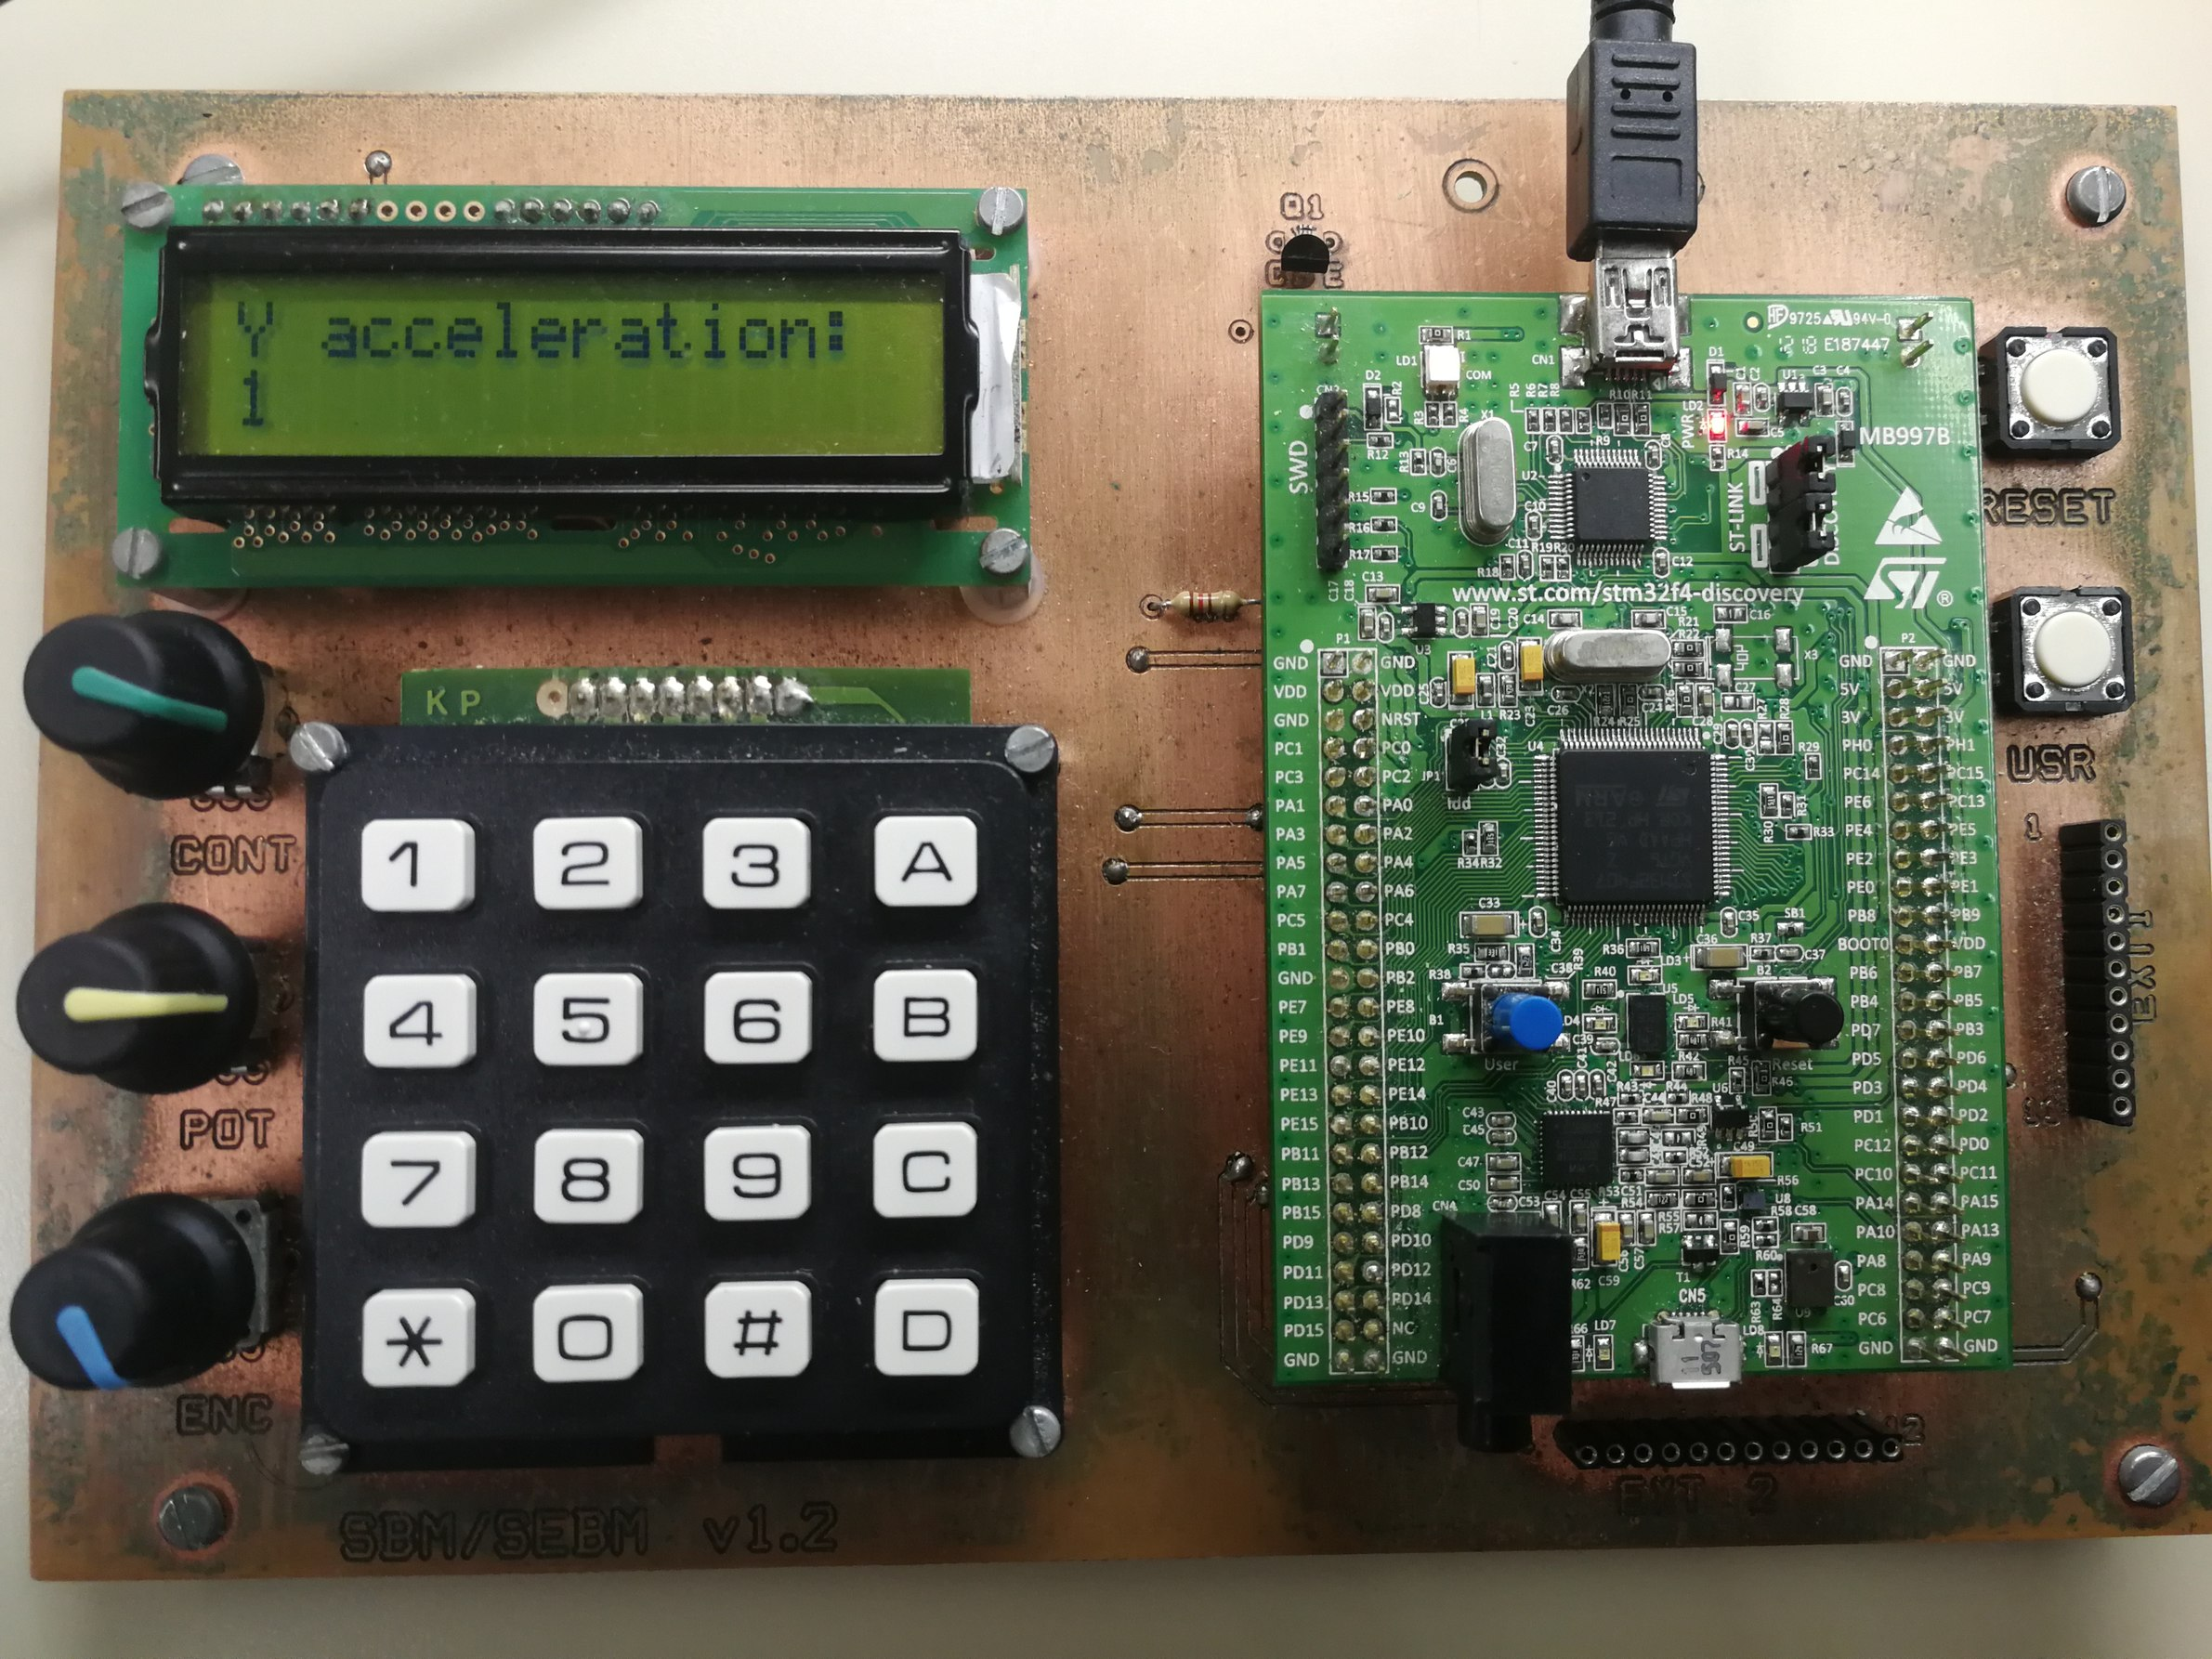
\includegraphics[width=.82\columnwidth]{../photos/board/p3-reading-initial_2}
  \caption{ \label{fig:p3-board-reading-initial} La placa mostrant el valor de l'acceleració Y, en repós. }
\end{figure}
\begin{figure}[p]
  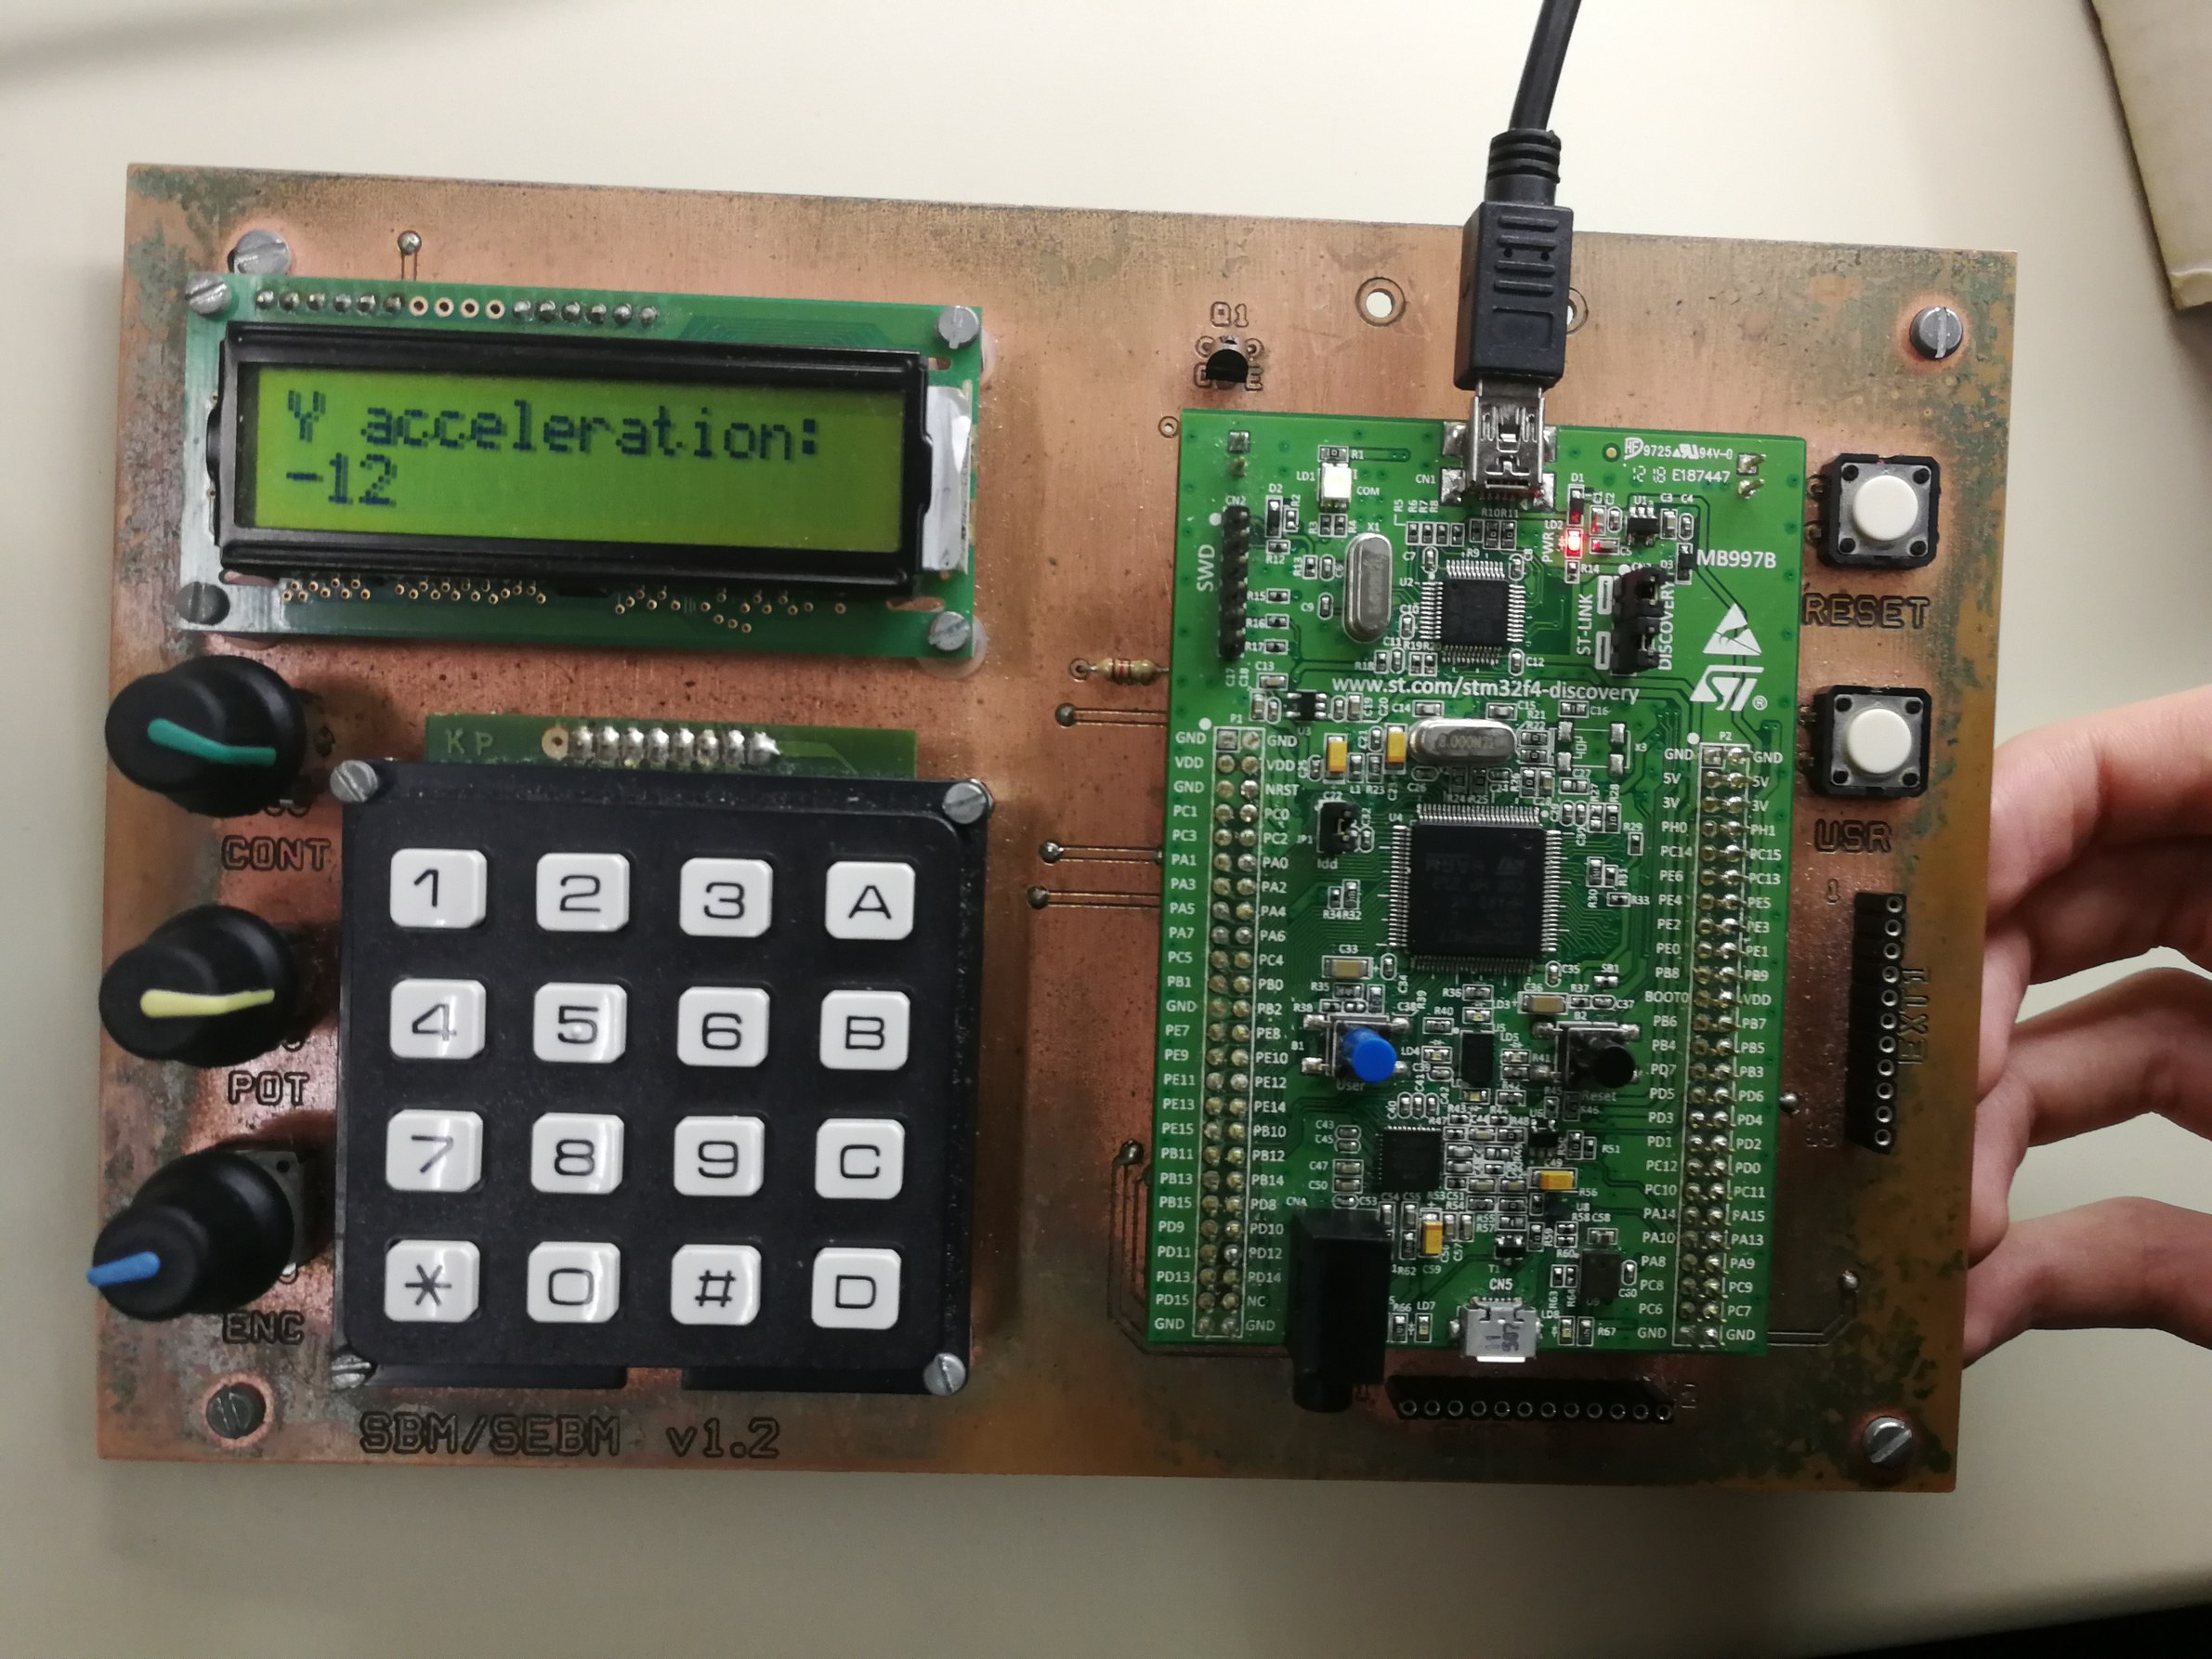
\includegraphics[width=.82\columnwidth]{../photos/board/p3-reading-tilt_2}
  \caption{ \label{fig:p3-board-reading-tilt} La placa mostrant el valor de l'acceleració Y, inclinada. }
\end{figure}

Comprovem que el programa funciona com s'espera. Aquests canvis conformen el
\commit{630531793ba43a7a78ff1f2ea68af3d0e6d139c4}.


\subsection{Programa final}

En aquesta última secció es demana escriure un programa que mostrarà l'acceleració en els
eixos X i Y periòdicament de forma gràfica. Ho farà dibuixant un asterisc a cada fila de
l'LCD (cada eix) indicant el valor relatiu de l'acceleració. En iniciar-se, la placa prendrà
el valor de l'acceleració com a zero (posició central). Els extrems de la pantalla representaran
aproximadament \SI{45}{\degree} de diferència en cada costat.

El programa s'implementa com segueix (estudi previ):

%previ
\begin{minted}[mathescape]{c}
// Acceleration value which maps to the first/last column in the LCD
#define DRAW_AXIS_SCALE 42
// Time to wait between refreshes
#define DRAW_AXIS_REFRESH 60
// Number of readings to average
#define DRAW_AXIS_AVG 6

inline int32_t clampColumn(int32_t col) {
    if (col < 0) return 0;
    if (col > 15) return 15;
    return col;
}

void accelDrawAxis(void) {
    // Initialize averaging buffers
    int32_t xacc_cache [DRAW_AXIS_AVG];
    int32_t yacc_cache [DRAW_AXIS_AVG];
    int32_t fill = 0, offset = 0;

    // Prepare LCD
    uint8_t bullet [] = {
        0b00000100,
        0b00000100,
        0b00001110,
        0b00011111,
        0b00011111,
        0b00001110,
        0b00000100,
        0b00000100,
    };
    LCD_ClearDisplay();
    LCD_Config(TRUE, FALSE, FALSE);
    LCD_Backlight(TRUE);
    LCD_CustomChar(2, bullet);

    // Read initial acceleration values
    int32_t xacc_0 = readAccel(LIS_R_OUT_X, 1);
    int32_t yacc_0 = readAccel(LIS_R_OUT_Y, 1);

    // Start the main loop
    while (1) {
        // Wait before reading
        SLEEP_MS(DRAW_AXIS_REFRESH);

        // Read acceleration on both axis, subtracted from initial
        int32_t xacc = readAccel(LIS_R_OUT_X, 1) - xacc_0;
        int32_t yacc = readAccel(LIS_R_OUT_Y, 1) - yacc_0;

        // Insert on buffers
        xacc_cache[offset] = xacc;
        yacc_cache[offset] = yacc;
        if (fill < DRAW_AXIS_AVG) fill++;

        // Get average value
        int32_t xacc_o = 0, yacc_o = 0, i;
        for (i = 0; i < fill; i++) {
            xacc_o += xacc_cache[(DRAW_AXIS_AVG + offset - i) % DRAW_AXIS_AVG];
            yacc_o += yacc_cache[(DRAW_AXIS_AVG + offset - i) % DRAW_AXIS_AVG];
        }
        xacc_o /= fill;
        yacc_o /= fill;

        // Move buffer slot
        offset = (offset + 1) % DRAW_AXIS_AVG;

        // Map acceleration to columns, and clamp
        // Formula: $\text{col} = \left \lfloor{ 15 \cdot \min(\max(x, 0), 1) }\right \rfloor$ where $x = \nicefrac{1}{2} \left(\frac{\text{acc}_o}{\text{DRAW\_AXIS\_SCALE}} + 1\right) $
        int32_t xcol = clampColumn((xacc_o + DRAW_AXIS_SCALE) * 15 / (DRAW_AXIS_SCALE * 2));
        int32_t ycol = clampColumn((yacc_o + DRAW_AXIS_SCALE) * 15 / (DRAW_AXIS_SCALE * 2));

        // (Re)draw screen
        LCD_ClearDisplay();
        LCD_GotoXY(xcol, 0);
        LCD_SendChar(2);
        LCD_GotoXY(ycol, 1);
        LCD_SendChar(2);
    }
}
\end{minted}
\vskip -1em
%/previ

\voluntari
S'ha definit un caràcter personalitzat (variable \mintinline{c}|bullet|)
per marcar el valor de cada acceleració.

\opcional
Per reduir les fluctuacions ocasionades pel soroll, es proposa fer una mitja temporal de les
últimes $N$ mostres i treballar amb la mitja. La variable $N$ (quantitat de mostres a promitjar)
s'anomena \mintinline{c}|DRAW_AXIS_AVG|.

\voluntari
Per ser encara més genèrics, s'ha estructurat el codi de forma que sigui fàcil multiplicar per
una \emph{finestra} a l'hora de processar els valors anteriors. %FIXME: extendre
%Per exemple, el codi actual seria
%equivalent a processar les mostres amb una finestra rectangular (mitja), però si volguéssim
%implementar una finestra de Hanning podriem definir-la:
%
%\begin{minted}{c}
%// Number of readings to average
%#define DRAW_AXIS_AVG 6
%// Average window
%static const int HANNING_WINDOW [] = {};
%\end{minted}
%\vskip -1em

Es modifica \fname{main} per cridar la funció \fname{accelDrawAxis} i es puja el programa
a la placa. El resultat pot veure's a les figures \ref{fig:p3-board-dots-initial} (estat
inicial, quan es pren el valor actual com a zero), i \ref{fig:p3-board-dots-tilt} (estat
quan s'inclina la placa en tots dos eixos.

\begin{figure}[p] %FIXME: subfigures?
  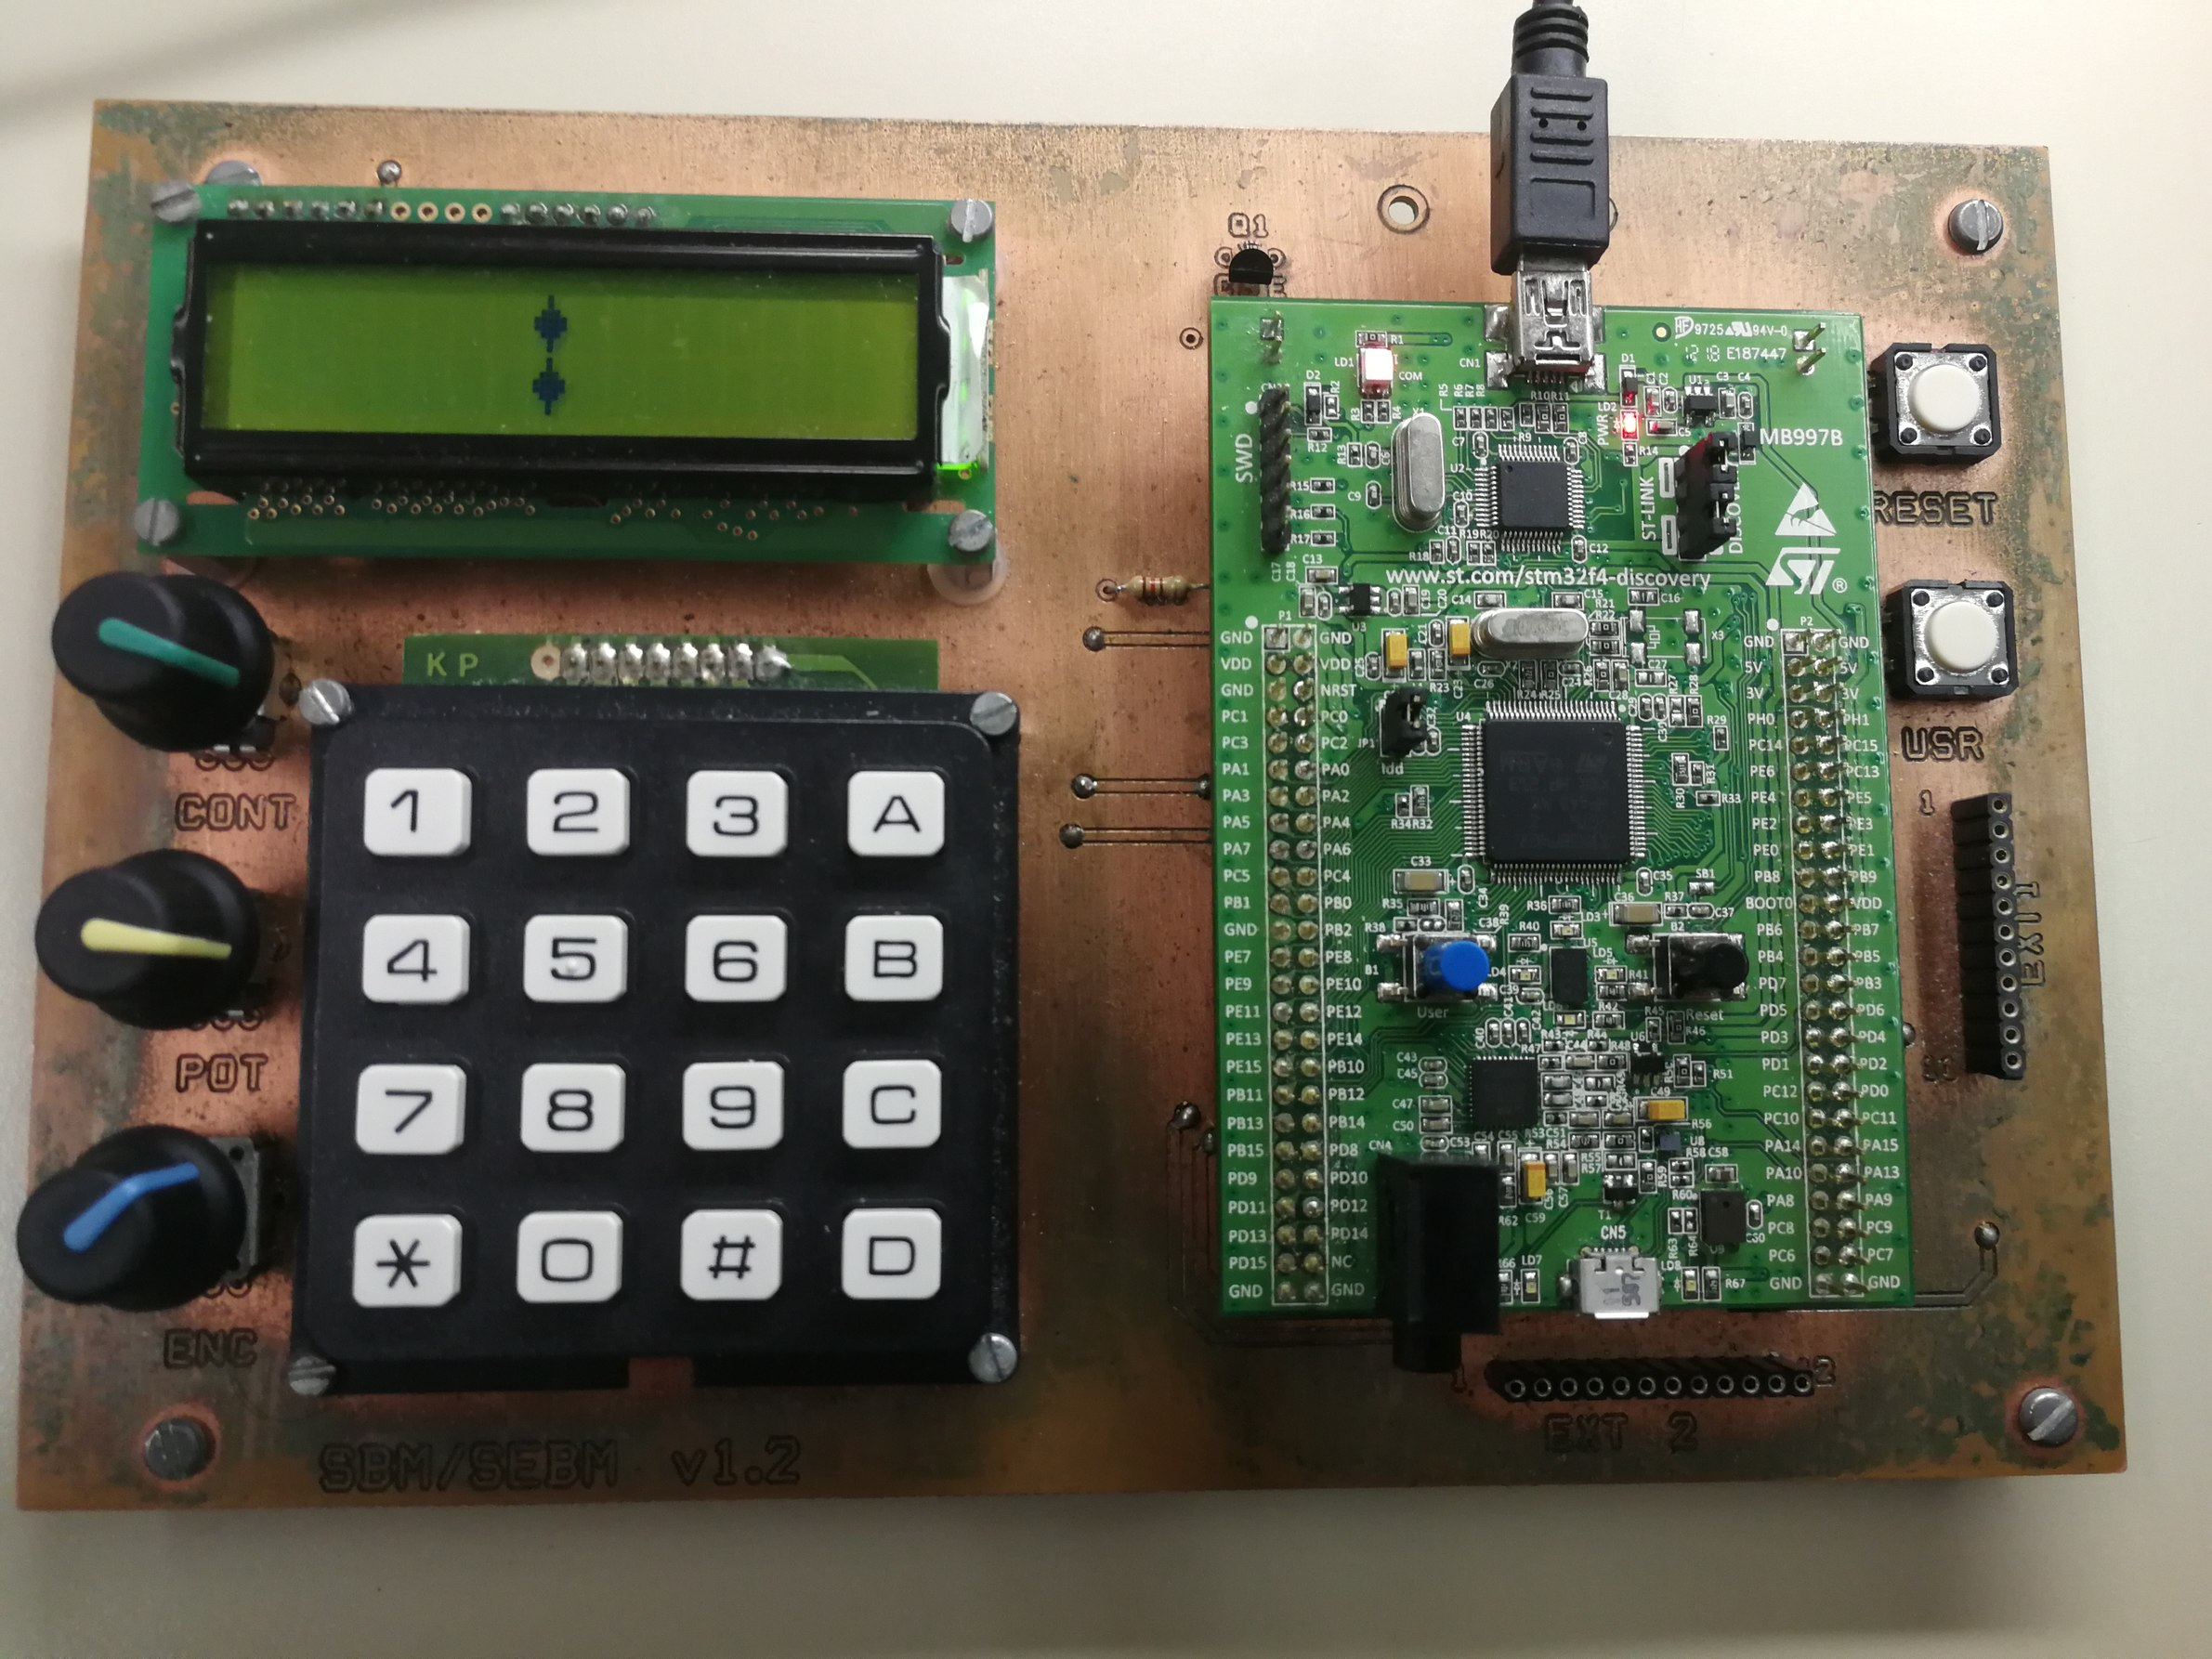
\includegraphics[width=.82\columnwidth]{../photos/board/p3-dots-initial}
  \caption{ \label{fig:p3-board-dots-initial} La placa mostrant l'acceleració gràficament, en repós. }
\end{figure}
\begin{figure}[p]
  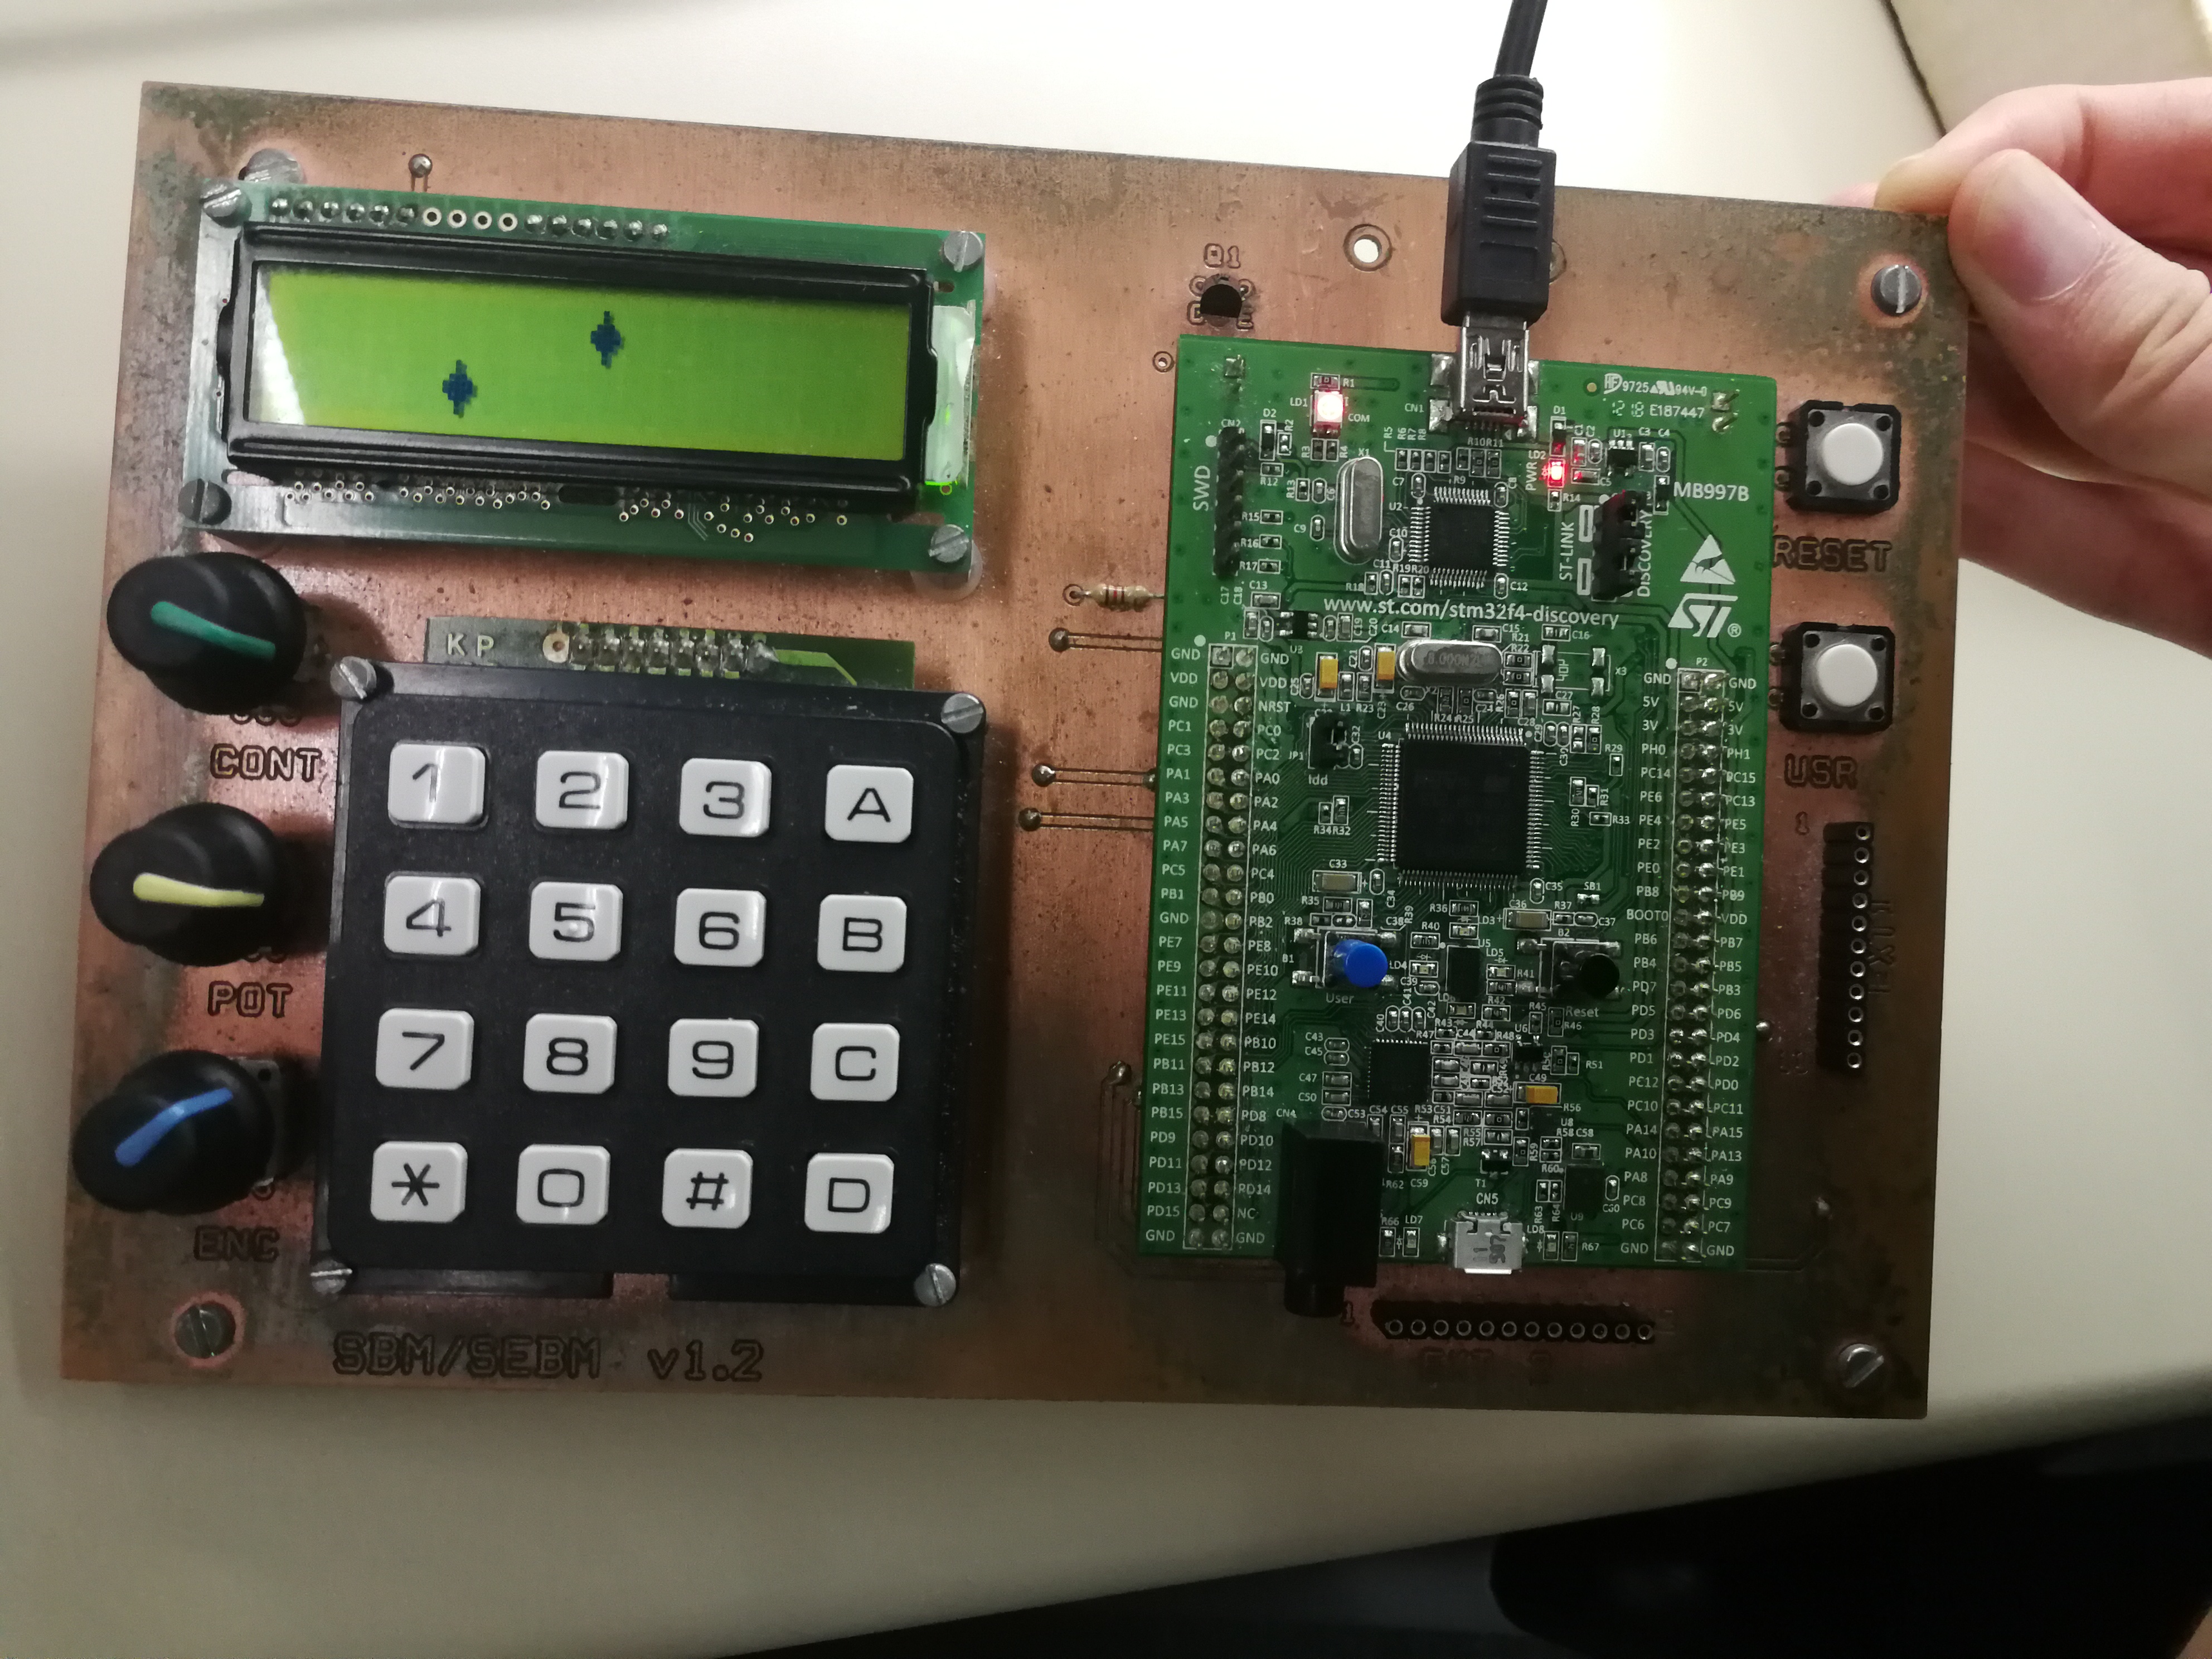
\includegraphics[width=.82\columnwidth]{../photos/board/p3-dots-tilt_1}
  \caption{ \label{fig:p3-board-dots-tilt} La placa mostrant l'acceleració gràficament, inclinada. }
\end{figure}

Es comprova el correcte funcionament del programa. Això conforma el
\commit{06ed1e2ebff859fecf3e91c35b615ce8fe56e918}.


\section{Conclusió}

La pràctica s'ha realitzat sense problemes, ha estat entretenida.
%FIXME: conclusion

\section{Ajustaments posteriors}

Més endavant s'ha vist oportú millorar el programa simple desenvolupat en la secció~\ref{sub:p3-whoami}
per incloure, a més del valor del registre, el model al que aquest correspon. S'ha implementat al \commit{09b749096ed89b047ecd95216da6d7d89336d165}:

\begin{minted}{diff}
--- a/main.c
+++ b/main.c
@@ -118,6 +118,7 @@ void accelWhoAmI(void) {
     LCD_GotoXY(0, 1);
     LCD_SendString("0x");
     LCD_SendString(valueStr);
+    LCD_SendString((value == 0x3B) ? " LIS302DL" : " LIS3DSH");
 
     while (1);
 }
\end{minted}
\vskip -1em

Cap altre canvi a destacar.
% TODO
